\documentclass[border=12pt]{standalone}
\usepackage[european]{circuitikz}
\begin{document}
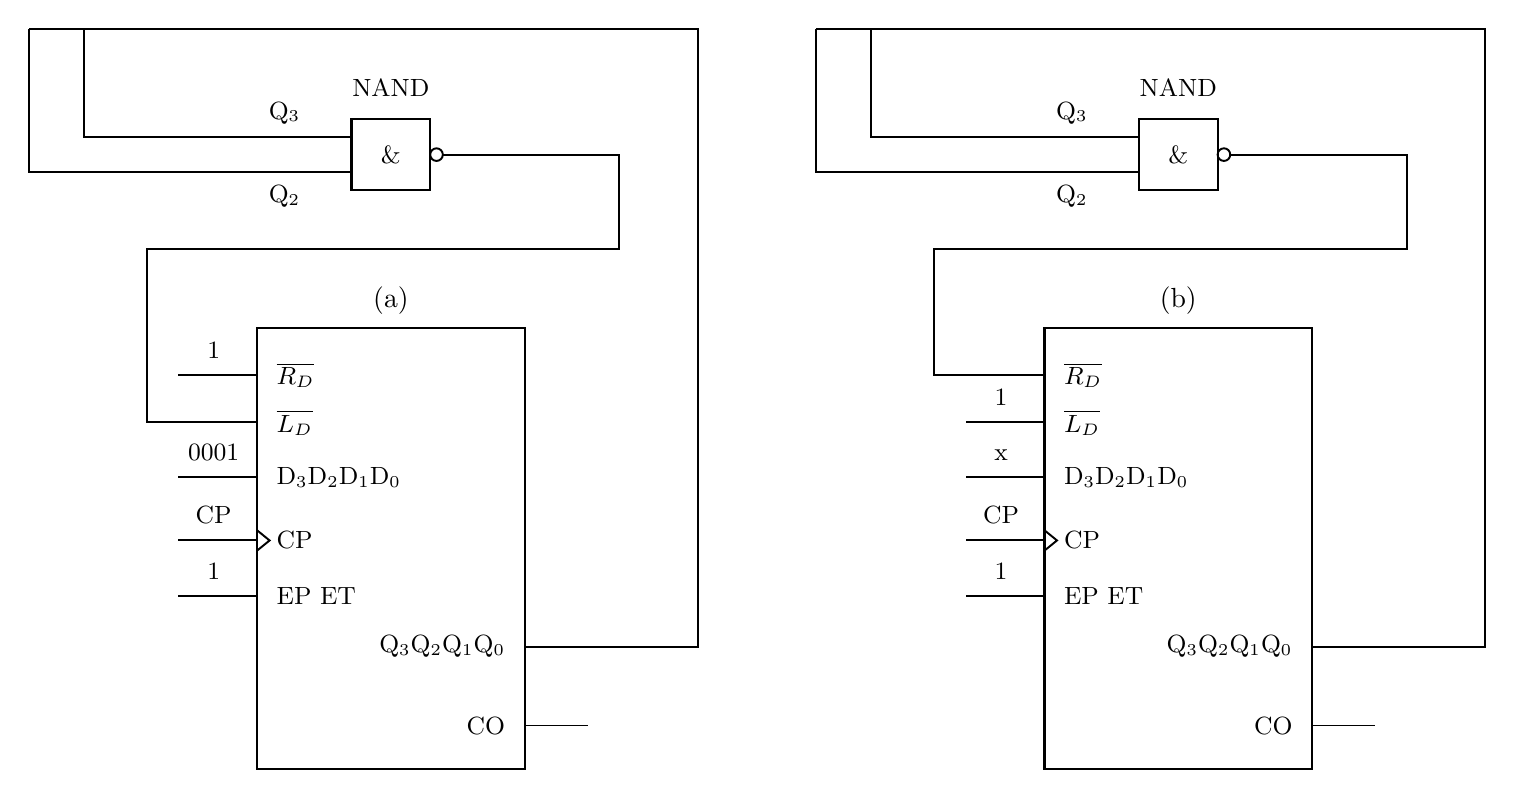
\begin{tikzpicture}[line width=0.7pt, font=\small]

% 74LS161 框 3.4 x 5.6；输入行 RD5.0 / LD4.4 / D3.7 / CP2.9 / EP·ET2.2
% 输出行 Q组1.55（画作总线）/ CO0.55
% 引脚电平标注一律写在该引脚线之上（不占左侧通道）
% 通道：NAND 输出下行 x=bx-1.4（在引脚端点 -1.0 之外）
%       NAND 输出起段 x=bx+4.6、Q 总线上行 x=bx+5.6、顶部横跨 y=9.4
%       NAND 两输入下行 x=bx-2.2（Q3）/ bx-2.9（Q2）
\newcommand{\sub}[3]{% #1 框左下 x  #2 子图号  #3 与非输出接入的输入行 y
  \draw[thick] (#1,0) rectangle (#1+3.4,5.6);
  \node[font=\normalsize] at (#1+1.7,5.95) {(#2)};
  \foreach \y/\n in {5.0/{$\overline{R_D}$},4.4/{$\overline{L_D}$},3.7/{D$_3$D$_2$D$_1$D$_0$},2.9/{CP},2.2/{EP ET}} {%
    \node[font=\small, anchor=west] at (#1+0.12,\y) {\n};
    \draw (#1,\y) -- (#1-1.0,\y);
  }
  \draw (#1,2.77) -- (#1,3.03) -- (#1+0.16,2.9) -- cycle;
  \node[font=\small, anchor=east] at (#1+3.28,1.55) {Q$_3$Q$_2$Q$_1$Q$_0$};
  \draw (#1+3.4,1.55) -- (#1+4.2,1.55);
  \node[font=\small, anchor=east] at (#1+3.28,0.55) {CO};
  \draw (#1+3.4,0.55) -- (#1+4.2,0.55);
  % 与非门
  \draw[thick] (#1+1.2,7.35) rectangle (#1+2.2,8.25);
  \node at (#1+1.7,7.8) {\&};
  \draw (#1+2.28,7.8) circle (0.08);
  \node[font=\small] at (#1+1.7,8.65) {NAND};
  % Q 总线 → 右上行 → 顶部左行 → 两条输入支路
  \draw (#1+4.2,1.55) -- (#1+5.6,1.55) -- (#1+5.6,9.4) -- (#1-2.9,9.4);
  \draw (#1-2.2,9.4) -- (#1-2.2,8.02) -- (#1+1.2,8.02);
  \draw (#1-2.9,9.4) -- (#1-2.9,7.58) -- (#1+1.2,7.58);
  \node[font=\small, anchor=south] at (#1+0.35,8.06) {Q$_3$};
  \node[font=\small, anchor=north] at (#1+0.35,7.54) {Q$_2$};
  % 与非输出 → 右下行 → 顶部左行 → 左通道下行 → 目标引脚
  \draw (#1+2.36,7.8) -- (#1+4.6,7.8) -- (#1+4.6,6.6) -- (#1-1.4,6.6) -- (#1-1.4,#3) -- (#1-1.0,#3);
}

\sub{0}{a}{4.4}
\node[font=\small, anchor=south] at (-0.55,5.08) {1};
\node[font=\small, anchor=south] at (-0.55,3.78) {0001};
\node[font=\small, anchor=south] at (-0.55,2.98) {CP};
\node[font=\small, anchor=south] at (-0.55,2.28) {1};

\sub{10.0}{b}{5.0}
\node[font=\small, anchor=south] at (9.45,4.48) {1};
\node[font=\small, anchor=south] at (9.45,2.98) {CP};
\node[font=\small, anchor=south] at (9.45,2.28) {1};
\node[font=\small, anchor=south] at (9.45,3.78) {x};

\end{tikzpicture}
\end{document}
